\begin{table}[H]
\centering
\definecolor{tabglobalgeneralnorm0}{rgb}{0.5845,0.0,0.149}
\definecolor{tabglobalgeneralnorm1}{rgb}{0.517,0.0,0.149}
\definecolor{tabglobalgeneralnorm2}{rgb}{0.5695,0.0,0.149}
\definecolor{tabglobalgeneralnorm3}{rgb}{0.502,0.0,0.149}
\definecolor{tabglobalgeneralnorm4}{rgb}{0.547,0.0,0.149}
\definecolor{tabglobalgeneralnorm5}{rgb}{0.607,0.0,0.149}
\definecolor{tabglobalgeneralnorm6}{rgb}{0.6295,0.0,0.149}
\definecolor{tabglobalgeneralnorm7}{rgb}{0.6596,0.0,0.149}
\definecolor{tabglobalgeneralnorm8}{rgb}{0.7979,0.0388,0.1341}
\definecolor{tabglobalgeneralnorm9}{rgb}{0.8025,0.042,0.1329}
\definecolor{tabglobalgeneralnorm10}{rgb}{0.8072,0.0452,0.1316}
\definecolor{tabglobalgeneralnorm11}{rgb}{0.9094,0.1419,0.1206}
\definecolor{tabglobalgeneralnorm12}{rgb}{0.891,0.1036,0.1102}
\definecolor{tabglobalgeneralnorm13}{rgb}{0.9889,0.3475,0.1766}
\definecolor{tabglobalgeneralnorm14}{rgb}{0.8493,0.074,0.1206}
\definecolor{tabglobalgeneralnorm15}{rgb}{0.9888,0.3398,0.1744}
\definecolor{tabglobalgeneralnorm16}{rgb}{0.8399,0.0676,0.123}
\definecolor{tabglobalgeneralnorm17}{rgb}{0.7932,0.0356,0.1353}
\definecolor{tabglobalgeneralnorm18}{rgb}{0.9893,0.3708,0.1833}
\definecolor{tabglobalgeneralnorm19}{rgb}{1.0,0.9801,0.7513}
\definecolor{tabglobalgeneralnorm20}{rgb}{1.0,0.9402,0.6538}
\definecolor{tabglobalgeneralnorm21}{rgb}{0.9984,0.8971,0.5596}
\definecolor{tabglobalgeneralnorm22}{rgb}{0.9961,0.8498,0.4615}
\definecolor{tabglobalgeneralnorm23}{rgb}{0.9961,0.7634,0.3684}
\definecolor{tabglobalgeneralnorm24}{rgb}{0.9955,0.6781,0.2894}
\definecolor{tabglobalgeneralnorm25}{rgb}{0.9933,0.5962,0.254}
\definecolor{tabglobalgeneralnorm26}{rgb}{0.991,0.4793,0.2143}
\definecolor{tabglobalgeneralnorm27}{rgb}{0.9463,0.2187,0.1412}
\definecolor{tabglobalgeneralnorm28}{rgb}{0.8867,0.0996,0.1107}
\definecolor{tabglobalgeneralnorm29}{rgb}{0.7046,0.0,0.149}
\begin{minipage}{0.78\textwidth}
\centering
\renewcommand{\arraystretch}{1.2}
\begin{tabular}{lccc}
\toprule
Checkpoint & First & Middle & Last \\
\midrule
0 & \cellcolor{tabglobalgeneralnorm0}\textcolor{white}{$0.408 \pm 0.047$} & \cellcolor{tabglobalgeneralnorm1}\textcolor{white}{$0.422 \pm 0.057$} & \cellcolor{tabglobalgeneralnorm0}\textcolor{white}{$0.408 \pm 0.047$} \\
1 & \cellcolor{tabglobalgeneralnorm2}\textcolor{white}{$0.412 \pm 0.046$} & \cellcolor{tabglobalgeneralnorm3}\textcolor{white}{$0.427 \pm 0.058$} & \cellcolor{tabglobalgeneralnorm4}\textcolor{white}{$0.417 \pm 0.046$} \\
5 & \cellcolor{tabglobalgeneralnorm5}\textcolor{white}{$0.402 \pm 0.059$} & \cellcolor{tabglobalgeneralnorm6}\textcolor{white}{$0.398 \pm 0.074$} & \cellcolor{tabglobalgeneralnorm7}\textcolor{white}{$0.392 \pm 0.060$} \\
15 & \cellcolor{tabglobalgeneralnorm8}\textcolor{white}{$0.353 \pm 0.061$} & \cellcolor{tabglobalgeneralnorm9}\textcolor{white}{$0.352 \pm 0.075$} & \cellcolor{tabglobalgeneralnorm10}\textcolor{white}{$0.350 \pm 0.060$} \\
50 & \cellcolor{tabglobalgeneralnorm11}\textcolor{white}{$0.310 \pm 0.058$} & \cellcolor{tabglobalgeneralnorm12}\textcolor{white}{$0.319 \pm 0.069$} & \cellcolor{tabglobalgeneralnorm13}\textcolor{white}{$0.258 \pm 0.055$} \\
200 & \cellcolor{tabglobalgeneralnorm14}\textcolor{white}{$0.334 \pm 0.058$} & \cellcolor{tabglobalgeneralnorm10}\textcolor{white}{$0.350 \pm 0.070$} & \cellcolor{tabglobalgeneralnorm15}\textcolor{white}{$0.259 \pm 0.055$} \\
last & \cellcolor{tabglobalgeneralnorm16}\textcolor{white}{$0.339 \pm 0.059$} & \cellcolor{tabglobalgeneralnorm17}\textcolor{white}{$0.355 \pm 0.071$} & \cellcolor{tabglobalgeneralnorm18}\textcolor{black}{$0.253 \pm 0.056$} \\
\bottomrule
\end{tabular}
\end{minipage}%
\hfill
\begin{minipage}{0.15\textwidth}
\centering
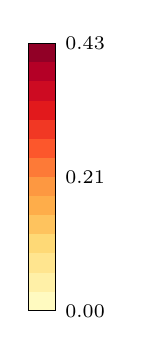
\begin{tikzpicture}
\fill[tabglobalgeneralnorm19] (0,0.0000) rectangle (0.35,0.2429);
\fill[tabglobalgeneralnorm20] (0,0.2429) rectangle (0.35,0.4857);
\fill[tabglobalgeneralnorm21] (0,0.4857) rectangle (0.35,0.7286);
\fill[tabglobalgeneralnorm22] (0,0.7286) rectangle (0.35,0.9714);
\fill[tabglobalgeneralnorm23] (0,0.9714) rectangle (0.35,1.2143);
\fill[tabglobalgeneralnorm24] (0,1.2143) rectangle (0.35,1.4571);
\fill[tabglobalgeneralnorm25] (0,1.4571) rectangle (0.35,1.7000);
\fill[tabglobalgeneralnorm26] (0,1.7000) rectangle (0.35,1.9429);
\fill[tabglobalgeneralnorm15] (0,1.9429) rectangle (0.35,2.1857);
\fill[tabglobalgeneralnorm27] (0,2.1857) rectangle (0.35,2.4286);
\fill[tabglobalgeneralnorm28] (0,2.4286) rectangle (0.35,2.6714);
\fill[tabglobalgeneralnorm9] (0,2.6714) rectangle (0.35,2.9143);
\fill[tabglobalgeneralnorm29] (0,2.9143) rectangle (0.35,3.1571);
\fill[tabglobalgeneralnorm2] (0,3.1571) rectangle (0.35,3.4000);
\draw[black,line width=0.3pt] (0,0) rectangle (0.35,3.4000);
\node[right,font=\scriptsize,anchor=west] at (0.35,3.4000) {0.43};
\node[right,font=\scriptsize,anchor=west] at (0.35,1.7000) {0.21};
\node[right,font=\scriptsize,anchor=west] at (0.35,0) {0.00};
\end{tikzpicture}
\end{minipage}
\caption{Global Wasserstein alignment, GeneralSheaf, normalised Laplacian, vs.\ topological reference. Mean $\pm$ SE across 10 datasets (First/Last), 8 for Middle (datasets with $L=2$ contribute no middle layer). (Pooled fold/layer SE averages 0.015 across cells; not shown per cell, see text.) Cell shading: white = 0, dark red = 0.43 (max value in this table), YlOrRd colormap, same scale as Fig.~\ref{fig: RM_Norm} etc.}
\label{tab:global_general_norm}
\end{table}
